\begin{figure*}[t]
    \centering
    \begin{minipage}[t]{0.49\textwidth}
        \centering
        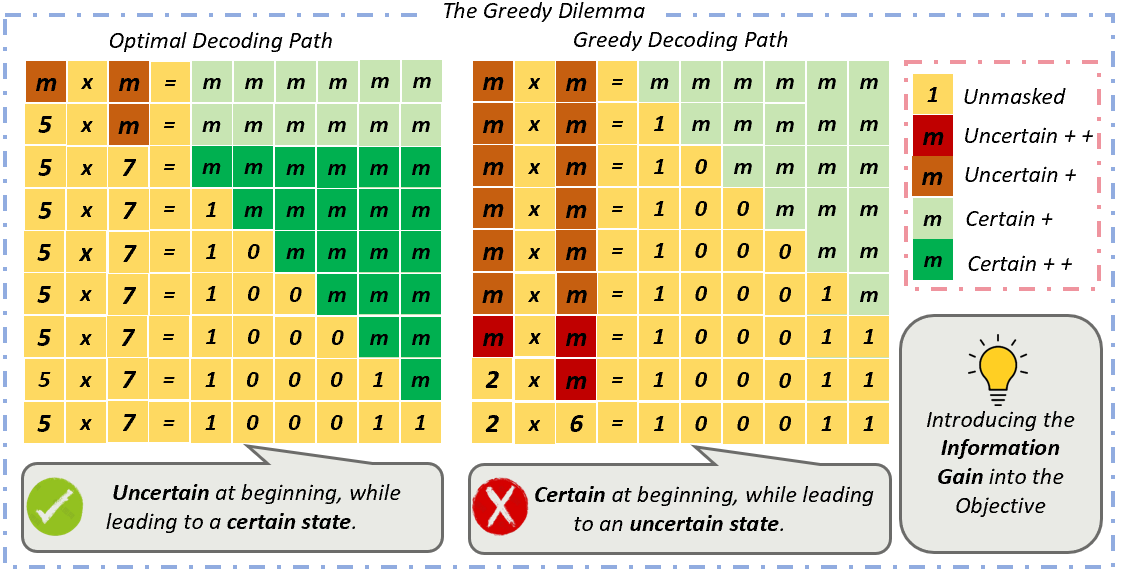
\includegraphics[width=\linewidth]{illustrative.png}
        \caption*{(a) The dilemma of greedy certainty-based sampling.}
        \label{fig:motivation}
    \end{minipage}
    \hfill
    \begin{minipage}[t]{0.49\textwidth}
        \centering
        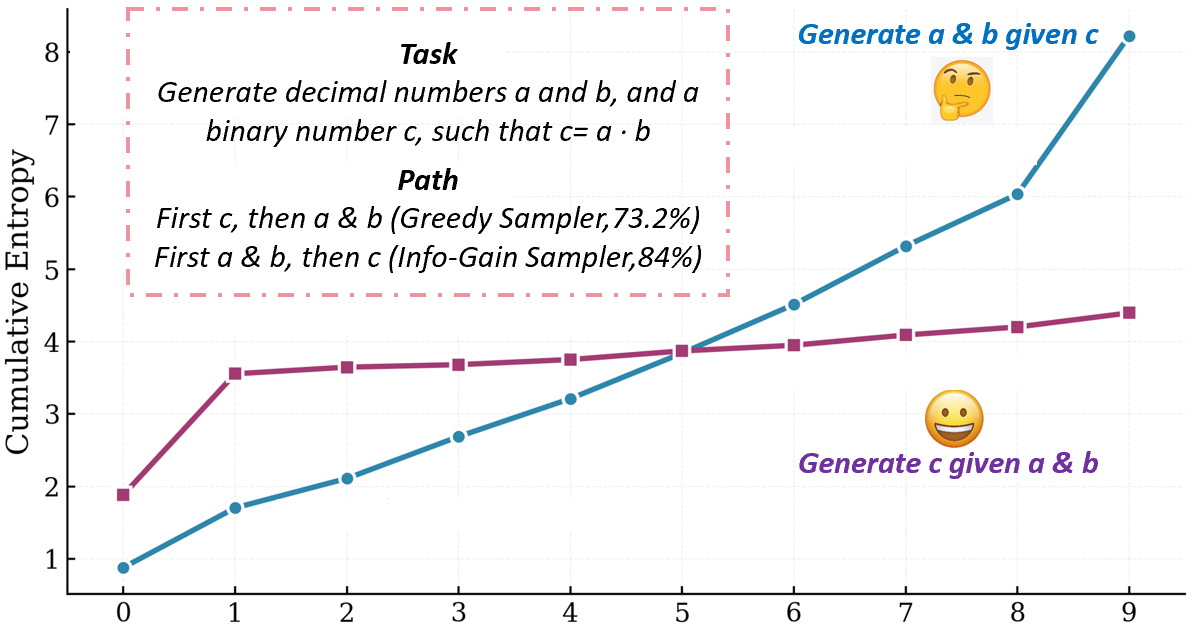
\includegraphics[width=\linewidth]{toy1-v4.png}
        \caption*{(b) Evolution of cumulative uncertainty.}
        \label{fig:toy_one_way}
    \end{minipage}

    \caption{
    \textbf{Motivation:} Analysis of decoding strategies on the one-way multiplication experiment.
    (a) Illustrates the contrast between the suboptimal path chosen by the greedy certainty-based sampler and the optimal path, motivating the introduction of the Info-Gain Sampler.
    (b) Shows the evolution of cumulative uncertainty throughout the decoding process.
    While the greedy sampler prioritizes decoding $c$ first (73.2\%) due to its immediate high confidence, it leads to failure because of the task's one-way nature.
    In contrast, the Info-Gain Sampler optimizes global uncertainty by resolving high-entropy factors $a$ or $b$ first (84.0\%), ensuring a successful decoding trajectory.
    }
    \label{fig:toy_analysis}
\end{figure*}
